\documentclass[10pt,twocolumn,letterpaper]{article}
\usepackage[review]{cvpr}
\usepackage{times,graphicx,amsmath,amssymb,booktabs,microtype,multirow}
\usepackage[accsupp]{axessibility}
\usepackage[pagebackref,breaklinks,colorlinks,allcolors=blue]{hyperref}
\def\paperID{-----}
\def\confName{CVPR}
\def\confYear{2027}
\newcommand{\R}{\mathbb{R}}
\newcommand{\norm}[1]{\left\lVert#1\right\rVert}
\title{A Finite-Event Audit of Decision and Temporal Fidelity\\in Graph-to-Spike Conversion}
\switchlinenumbers*
\author{Anonymous authors}
\begin{document}
\maketitle
\begin{abstract}
Reconstruction error is a convenient proxy for ANN-to-SNN conversion, but it does not say whether a graph classifier preserves its decision. We audit two finite-event invariants in frozen superpixel graph classifiers. First, legal one-event changes that reduce actual graph-message error worsen the teacher-class margin in 40.9\% and 31.9\% of message-improving interventions on MNIST and CIFAR10. The rates describe these intervention distributions: the effect persists under coordinate and residual selection rules, with larger adverse rates for residual selection. Second, exchanging legal two-tick codewords with bitwise-equal local decoded tensors and equal local event counts changes downstream predictions and whole-network activity. These exchanges do not control first-prefix profile or absolute amplitude. A directional margin analysis and an executable source recurrence explain why message error and matched local endpoints omit signed decision direction and downstream state history. The controlled counterexamples motivate reporting decisions at every required prefix, the intervention rule and eligible set, and whole-network activity.
\end{abstract}

\section{Introduction}
A finite event can improve a reconstruction metric and still move a graph classifier toward the wrong class. In a visual superpixel graph, a one-level change to a single event can reduce the next-message error while reversing the teacher-class margin. A different finite-event change can preserve a local decoded endpoint exactly and still alter the trajectory delivered to later layers. These two cases expose a basic question: which downstream quantities does local reconstruction actually preserve?

ANN-to-SNN conversion approximates a pretrained network without retraining its weights. Calibration, bias correction, and differential coding support high fidelity at short prefixes~\cite{li2021,wu2024ftbc,huang2025}. Our graph adaptations follow this pattern: four active ticks approximately preserve the accuracy of three independently trained teachers on fixed and gated superpixel networks, while one tick leaves a clear gap. That short-prefix regime makes the preserved quantities testable.

Two forms of information loss are relevant. Next-message error uses the actual adjacency and weights, yet its norm discards the perturbation's direction relative to class boundaries. Exact local terminal reconstruction preserves the decoded value, but omits the intermediate states encountered by downstream event units. A correction can therefore reduce message error while moving the final decision toward a competing class; a code can match its local endpoint while changing the downstream trajectory.

We test these distinctions through controlled hard-event interventions in frozen graph classifiers. The primary setting is MNIST and CIFAR10 superpixel classification with residual GCNs. A complementary GatedGCN study examines residual centering, while classical node classification supplies context for propagation and readout effects. Prediction agreement measures fidelity to the teacher; ground-truth accuracy measures task performance. Local event counts and whole-network cost are reported separately.

The central finding is therefore: \emph{improving a local reconstruction metric need not preserve the downstream decision, and matching a local terminal reconstruction need not preserve the computation that produces it}. In the spatial experiment, legal one-event changes that reduce immediate message MSE worsen the teacher-class margin in 332/811 MNIST and 296/928 CIFAR10 cases. In the temporal experiment, two codewords with identical local two-tick decoding and equal local event counts change downstream predictions and whole-network activity when exchanged. A three-teacher continuous diagnostic localizes the largest single-site one-tick sensitivity to the first node activation: recovering it closes 54.1\% and 23.5\% of the teacher-disagreement gap, compared with 8.8\% and 14.9\% for both readout sites.

The contribution is a controlled finite-event audit of one frozen graph computation. Directional class margins connect graph-propagated errors to classification, and exact local codeword equivalences expose temporal-prefix history under a matched endpoint and event count. These tests support a reporting consequence: assess decisions at every required prefix, report the intervention rule and eligible set, and account for whole-network activity after each realizable intervention.

\begin{figure}[t]
\centering
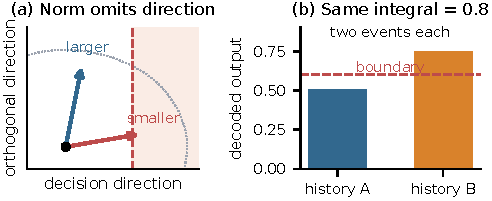
\includegraphics[width=\linewidth]{figures/concept.pdf}
\caption{Two information losses in reconstruction metrics. Left: a smaller error norm can cross a decision boundary when its direction changes (schematic). Right: two input histories have identical integrated input and two emitted events, but the fixed source neuron decodes them differently. The temporal values are an executable recurrence counterexample, rather than a dataset estimate.}
\label{fig:concept}
\end{figure}

\section{Related Work}
\paragraph{Conversion, calibration, and readout.}
Calibration methods correct systematic approximation errors in converted networks: layerwise calibration matches pretrained ANN responses~\cite{li2021}, while distribution-based threshold and potential initialization, forward temporal bias correction, and error-aware parameter calibration address related mismatches~\cite{bojkovic2024,wu2024ftbc,li2024erroraware}. Readout addresses a complementary loss: retaining the final membrane residual preserves information discarded by integer spike counts, including under uneven arrivals~\cite{hao2023residual}. This distinction motivates our early node experiments separating hidden approximation from output quantization.

Event-level coding and timing determine what a consumer sees within a finite prefix. Differential coding with graded units and spiking neurons (DCGS) transmits activation changes and supplies a threshold-iteration procedure~\cite{huang2025}; its public event unit underlies the graph adaptations studied here. One-Spike SNN is a single-spike phase-coding converter that also demonstrates GCN conversion~\cite{hwang2025onespike}; our one-event changes are diagnostic interventions inside a DCGS-derived adapter and are neither an implementation of nor a matched comparison against that converter. Temporal-misalignment research shows that event order affects low-latency conversion~\cite{bojkovic2025}, and closed-loop feature/output alignment has been studied at short horizons~\cite{li2026cka}.

Decision-aware objectives use downstream predictions to choose quantization parameters. PD-Quant optimizes quantization parameters using prediction differences rather than layerwise reconstruction~\cite{liu2023pdquant}; we change no quantization parameter or calibration rule and instead ask which exact local invariants fail to determine downstream behavior. Collectively, these works establish that reconstruction, decisions, and event timing are distinct concerns. Our experiment asks a narrower graph-specific question: inside a frozen graph event converter, does exact terminal equality at a local site, together with an equal local event count, preserve downstream decisions and whole-network activity?

\paragraph{Graph-dependent approximation.}
Degree-Quant studies quantization-aware graph training, and A$^2$Q incorporates aggregation into quantization design~\cite{degreequant2021,a2q2023}. Both account for structural effects on approximation. We examine a related issue in a frozen converted computation: the relationship between immediate message fidelity and the final decision. Feature-only and permuted-operator controls isolate the role of the actual propagation operator while preserving the task graph and fitting budget. The visual models and data follow Benchmarking GNNs~\cite{dwivedi2023}. Static propagation, feature-dependent gating, and classical node classification use different operators and codes and are analyzed separately.

\section{Analysis and Experimental Design}
\subsection{Frozen graph computation and event semantics}
Our primary teacher has four residual graph-convolution layers of width 146. For fixed normalized adjacency $A$, its evaluation-mode layer is
\begin{equation}
 H_{\ell+1}=H_\ell+\operatorname{ReLU}(AH_\ell W_\ell^\top+b_\ell),
 \label{eq:block}
\end{equation}
with batch normalization folded into $W_\ell,b_\ell$. Node features and positions are embedded together. Mean pooling feeds a 146--73--36--10 MLP with two hidden ReLUs. The conversion has four node activation sites and two readout sites. Its graph operator weights each original directed edge $u\!\to\!v$ by $[\max(d_{\rm out}(u),1)\max(d_{\rm in}(v),1)]^{-1/2}$, without adding self-loops. The residual path supplies the identity connection.

An event is a signed scalar from $\{0,\pm\theta,\ldots,\pm\theta/128\}$, with per-channel threshold $\theta>0$. It is not a binary spike. We call the total number of nonzero scalar events across the network \emph{whole-network activity}; this quantity is distinct from effective spike count, delivered weight, memory traffic, latency, and energy. Let $c_t$ be the current at active tick $t$, and let $(v,C,a,b)$ denote membrane, cumulative output, integrated input, and integrated output states. The source differential unit first computes
\begin{equation}
 m=v+c_t+a-b,\qquad \widetilde C=C+b.
\end{equation}
It emits the largest eligible magnitude $s_t$. A positive level $q=\theta2^{-k}$ requires $m\geq0.75q$; a negative level requires $m\leq-0.75q$ and $\widetilde C\geq q$. The updates are
\begin{equation}
\begin{split}
 v&\leftarrow m-s_t,\quad C\leftarrow\widetilde C+s_t,\\
 a&\leftarrow a+c_t/t,\quad b\leftarrow b+s_t/t.
\end{split}\label{eq:state}
\end{equation}
The decoder is $D_T(s)=\sum_{t=1}^T s_t/t$. Raw inputs and affine biases enter once, at the first active tick. We use $T$ for active ticks, not measured latency. Residual and readout arithmetic remains continuous where specified by the adapter.

\subsection{What a graph message norm does not determine}
For an activation perturbation $E$ at a fixed site, the immediate next-message perturbation is exactly
\begin{equation}
 \Delta M=AEW^\top.\label{eq:message}
\end{equation}
Consequently, $\norm{\Delta M}_F^2$ accounts for the actual propagation operator, but compresses a signed, graph-dependent perturbation to one scalar. A two-layer classifier with linear graph readout $R$ gives the particularly transparent relation $\Delta z=RAEW^\top$. This identity is elementary linear algebra. Its value here is to expose which information a norm omits.

Let $y=\arg\max_k z_k$ be the teacher class, and define its margin against every competitor $k\ne y$ by $m_k=z_y-z_k$. The converted prediction agrees with $y$ precisely when
\begin{equation}
 m_k+\Delta z_y-\Delta z_k>0\quad\text{for all }k\ne y,
 \label{eq:margin}
\end{equation}
apart from ties. In a linear downstream region, write $\Delta z=J\operatorname{vec}(E)$, with $J$ including the graph and readout. Then the relevant perturbations are the signed projections
\begin{equation}
 (J_y-J_k)\operatorname{vec}(E),
\end{equation}
rather than the reconstruction norm alone. A sufficient condition is
\begin{equation}
 \norm{\operatorname{vec}(E)}_2<
 \min_{k\ne y}\frac{m_k}{\norm{J_y-J_k}_2},\label{eq:sufficient}
\end{equation}
with zero rows imposing no restriction. Smaller norms tighten this worst-case bound; they do not order two actual errors pointing in different directions. In the full converted network, later event boundaries can also change $J$ or invalidate a fixed-region linearization. We therefore use Eq.~\eqref{eq:margin} as an exact decision condition and test message interventions with the actual hard forward pass.

For reported interventions, the scalar teacher-class margin is the converted logit of $y$ minus the largest converted competing logit. The competing class can change after intervention. Fixing the teacher's original runner-up can miss a newly dominant class. Ground-truth accuracy answers a different question: a converted prediction can disagree with an incorrect teacher and become correct. We retain both metrics instead of treating improved accuracy as evidence of improved conversion fidelity.

This perspective connects to early node-conversion analysis. Under nonsaturating constant-drive IF coding, rate error scales with $\theta/T$; retaining the membrane residual removes the final count quantization. Combining a valid hidden-error envelope with Eq.~\eqref{eq:sufficient} gives a sufficient time budget depending on propagation and margin. It does not imply that a common time budget, global bias sign, or row-stochastic bound applies to every graph. Symmetric degree normalization is not generally row stochastic. The supplementary material gives the readout identity, assumptions, and historical node results.

\subsection{What terminal reconstruction does not determine}
Equation~\eqref{eq:state} stores more than a decoded terminal activation. Replacing a first-tick event by $s_1+\delta$ must also change $v\leftarrow v-\delta$, $C\leftarrow C+\delta$, and $b\leftarrow b+\delta$. A later event consequently depends on both the incoming history and state. Matching $D_T(s)$ at one site cannot by itself match the intermediate currents received at its consumers.

A scalar counterexample uses exactly the frozen source recurrence, $\theta=1$, zero initial state, and $T=2$. The input histories $(c_1,c_2)=(0.01,1.58)$ and $(1,-0.4)$ have the same integrated input $c_1+c_2/2=0.8$. Both emit two nonzero events. Yet the decoded outputs are $0.5078125$ and $0.75$. A fixed decision boundary at $0.6$ separates them (Fig.~\ref{fig:concept}). Thus equality of integrated input, alphabet, time budget, and event count does not determine a nonlinear consumer's decoded result.

To test the same issue inside real graphs, we use source-verified first-site codeword pairs
\begin{equation}
 (q,-q/2)\quad\longleftrightarrow\quad(q/2,q/2).
 \label{eq:words}
\end{equation}
Both decode to $3q/4$ and contain two events (Fig.~\ref{fig:temporal-mechanism}). They differ in first-prefix profile and in unweighted absolute amplitude: the unweighted magnitudes sum to $3q/2$ and $q$, respectively. We apply a replacement only when all levels belong to the original alphabet and actual source replay under the known zero second-tick input produces the required second event. Both directions are checked; the subsequent forward pass executes normally. This is an exact local equivalence test, not a proposed efficient encoder. Equality at every consumed tick, together with identical initial state, would preserve a deterministic downstream trajectory by induction. Equality only at its terminal tick is weaker. This is consistent with prior temporal-misalignment results~\cite{bojkovic2025}; our diagnostic tests terminal equality together with fixed local event count inside the graph adapter, while leaving absolute amplitude and the first-prefix profile uncontrolled.

\begin{figure}[t]
\centering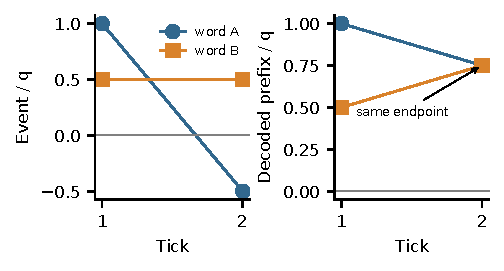
\includegraphics[width=\linewidth]{figures/temporal_mechanism.pdf}
\caption{The local equivalence test. Two legal codewords have two nonzero events and the same decoded endpoint $3q/4$, but present different first-prefix values to downstream consumers. Source replay verifies eligibility before replacement; the rest of the network is then executed without resetting its states.}
\label{fig:temporal-mechanism}
\end{figure}

\subsection{Interventions, controls, and evidence scope}
We use three complementary evidence levels. First, full historical official test predictions from three teacher seeds characterize conversion fidelity, and full validation position interventions localize error. Second, single-teacher hard interventions and calibration comparisons use 512 fixed, previously exposed validation graphs per task. Third, exact temporal-code tests use 128 training graphs per task, and the centered-residual profiles use all 45,000 CIFAR10 training graphs for one GatedGCN teacher. These splits serve different purposes. Official validation and test sets were exposed during earlier development; their results are descriptive evidence, not new blind confirmation.

For position analysis, an ideal causal ReLU replaces one selected converted activation while leaving the graph, weights, and incoming converted computation fixed. It is a continuous diagnostic. Restoring all six sites reproduces the ANN; an empty intervention reproduces the conversion. Group effects are nonadditive because interventions alter subsequent computation.

For hard intervention, we modify one existing nonzero first-site event up or down one legal amplitude level, update all affected states, and replay the network. Two label-free coordinate rules are used: a deterministic coordinate and the largest eligible local residual. The eligible coordinate sets can differ between upward and downward moves. Each task yields four attempts per graph, or 2,048 first-tick interventions. The teacher is used only afterward to measure margin and agreement. Confidence intervals resample graphs, retaining their repeated interventions together.

Calibration controls share teacher weights, histogram thresholds, 512 training graphs, 693 initial-potential offsets, and 64 Adam updates. The offsets are $\theta\rho$ with $\rho\in[-0.5,0.5]$. Local fitting averages normalized site MSE; graph-output fitting targets teacher logits; their mixture uses both. A second control family fits an immediate-message objective and compares actual $A$ with identity and within-graph conjugation $P^{-1}AP$. The graph used for the task is unchanged. We also retain the source 100-step threshold iteration and fallback rules as a graph adaptation; its placement, eight-level setting, and calibration horizon are specified separately in the supplement.

\section{Results}
\subsection{High fidelity and a concentrated short-prefix bottleneck}
Fidelity at longer prefixes is high, but it does not resolve the first-tick gap. At four or eight ticks (Table~\ref{tab:main}), the adapted differential code closely matches teacher accuracy on both fixed GCNs and the stronger CIFAR10 GatedGCN. The latter retains continuous gates, products, normalization, and readout; its high fidelity therefore demonstrates a hybrid graph adaptation with event placement different from the fixed-GCN experiment.

\begin{table}[t]
\caption{Historical full-test accuracy (\%), mean $\pm$ sample SD over three teacher seeds on the same 10,000 graphs. The tests were previously exposed. GatedGCN is a separate hybrid adapter with continuous gates; the table establishes fidelity, not superiority of a new method.}
\label{tab:main}
\centering\small
\setlength{\tabcolsep}{3.5pt}
\begin{tabular}{lrrr}\toprule
Task / teacher & ANN & $T=4$ & $T=8$\\\midrule
MNIST / GCN & $91.02\pm.27$ & $91.05\pm.26$ & $91.02\pm.26$\\
CIFAR10 / GCN & $54.94\pm.07$ & $54.92\pm.08$ & $54.97\pm.05$\\
CIFAR10 / Gated & $68.77\pm.41$ & $68.75\pm.33$ & $68.76\pm.39$\\\bottomrule
\end{tabular}
\end{table}

Position interventions localize the short-prefix gap to the first node site. At one tick, fixed-GCN conversion falls to $71.44\pm2.80\%$ on MNIST and $46.80\pm1.22\%$ on CIFAR10. On the full 5,000-graph validation split for each teacher, restoring the first node site closes 54.08\% and 23.54\% of the teacher-disagreement gap, measured per teacher and then averaged. Restoring all four node sites closes 80.4\% and 45.2\%; the two readout sites close 8.8\% and 14.9\%. The first site is the largest single-site accuracy recovery on both tasks. This recovery measures conditional sensitivity using a continuous response without finite-event constraints.

\begin{figure}[t]
\centering
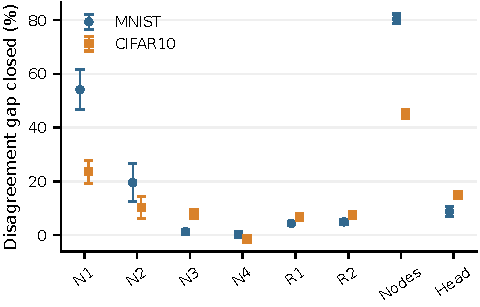
\includegraphics[width=\linewidth]{figures/position_recovery.pdf}
\caption{First-site recovery at $T=1$ dominates the conditional one-tick sensitivity. Gap closure is the recovered fraction of teacher disagreement on full, previously exposed validation data, averaged across three teachers; sample SD is shown. Node and readout groups restore four and two sites and are nonadditive.}
\label{fig:positions}
\end{figure}

Classical node classification provides a compatible but distinct observation. Audited historical two-layer IF experiments approach their own ANN teachers at longer horizons when analytic bias compensation and membrane readout are used. For example, Cora reaches 80.16\% at $T=8$ against an 80.46\% teacher. The decoder and time scale differ from Table~\ref{tab:main}; supplementary results retain this separation rather than pooling the two as one converter.

\subsection{A better message can have a worse decision direction}
Message improvement does not order downstream decision quality. On MNIST, 811 of 2,048 interventions reduce the actual first-tick next-message MSE; 332 worsen the teacher-class margin (40.94\%, graph-cluster bootstrap 95\% interval [37.28,44.57]\%). On CIFAR10, the corresponding count is 296 of 928 (31.90\% [28.66,35.31]\%). The same first-tick modifications worsen the $T=2$ margin in 48.71\% and 44.07\% of message-improving cases. These later percentages retain the first-tick message condition; the rates are conditional on the intervention distribution and are not conversion-wide frequencies.

\begin{table}[t]
\caption{Lowering first-tick message MSE can worsen the teacher-class margin. Rates use the same first-tick MSE condition at $T=1$ and $T=2$, with 512 graphs and 2,048 attempts per task and 95\% graph-cluster bootstrap intervals.}
\label{tab:hard}\centering\small\setlength{\tabcolsep}{3pt}
\begin{tabular}{llrl}\toprule
Task & Readout & Adverse / improved & Rate [interval] (\%)\\\midrule
MNIST & $T=1$ & 332 / 811 & 40.94 [37.28,44.57]\\
 & $T=2$ & 395 / 811 & 48.71 [45.02,52.42]\\
CIFAR10 & $T=1$ & 296 / 928 & 31.90 [28.66,35.31]\\
 & $T=2$ & 409 / 928 & 44.07 [40.54,47.60]\\\bottomrule
\end{tabular}\end{table}

The mismatch also occurs in one teacher example with a large top-two margin. On MNIST validation graph 437, the teacher and ground truth are class 5, and the teacher's top-two margin is 5.20378. A deterministic downward event change reduces message MSE from 0.00604723 to 0.00604511, while the converted teacher-class margin changes from 1.97242 to $-3.74764$, flipping its prediction from 5 to 4. The message norm improves, but Eq.~\eqref{eq:margin} fails for the perturbed decision.

The adverse rate is present under every selection rule, but its magnitude depends on which eligible event changes. Figure~\ref{fig:hard-strat} separates two label-free coordinate rules and two amplitude directions at $T=1$: on MNIST the adverse rate is 30.6--36.2\% under deterministic coordinates and 48.5--49.0\% under largest-residual selection, with corresponding CIFAR10 ranges of 20.4--24.7\% and 38.5--42.6\%. At the graph level, 50.2\% of MNIST and 42.2\% of CIFAR10 graphs have at least one adverse message-improving intervention, and 7.8\%/12.7\% have at least one resulting prediction change under these fixed rules.

\begin{figure}[t]
\centering
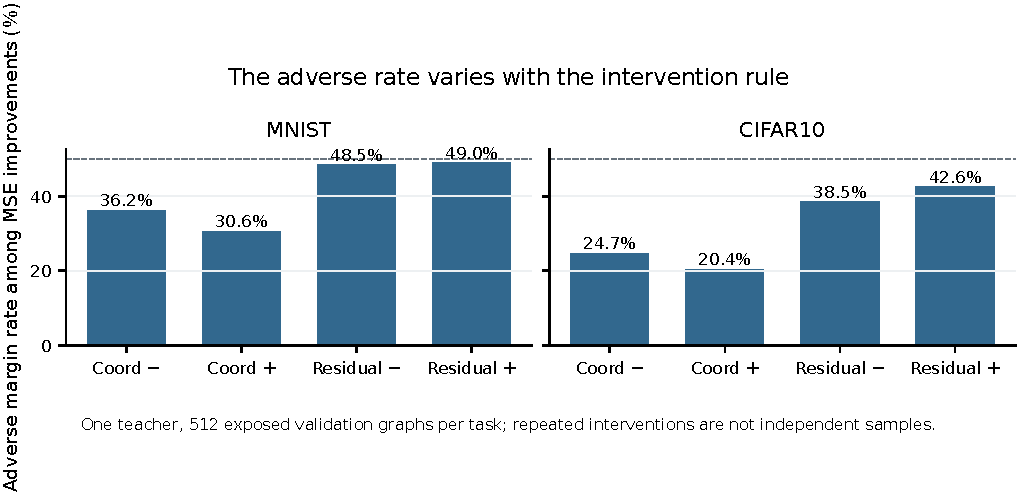
\includegraphics[width=\linewidth]{figures/hard_intervention_stratified.pdf}
\caption{Largest-residual selection has higher adverse rates than deterministic coordinates in every direction stratum at $T=1$. One teacher and 512 exposed validation graphs per task; repeated interventions are not independent samples.}
\label{fig:hard-strat}
\end{figure}

Finite residual allocation exhibits the same distinction. Compared with local allocation, actual-message allocation reduces normalized message MSE from 0.001378 to 0.001280 on MNIST and from 0.002018 to 0.001717 on CIFAR10. On CIFAR10, 491 of 512 graphs improve this metric, yet 27 of those change from correct to incorrect. The corresponding MNIST counts are 440 and 17. Gains on other graphs can offset these losses in aggregate accuracy, so an improved mean can coexist with adverse individual decisions. These policies share extra event opportunities; their realized event counts can differ.

\subsection{Sensitivity does not select a superior calibration target}
Calibration targets do not show a consistent decision advantage under matched resources (Table~\ref{tab:calibration}). Local calibration already recovers much of the one-tick accuracy gap. Switching to graph-output or mixed fitting produces small, setting-dependent changes: output-minus-local differences on full historical tests are $+0.20/+0.18$ percentage points at MNIST $T=1/2$, and $-0.18/+0.19$ on CIFAR10. Full-validation differences are $-0.10/-0.13$ and $-0.27/+0.43$. None of the tested objectives shows a consistent advantage, and these differences do not isolate an optimal correction target.

\begin{table}[t]
\caption{Matched local, output, and mixed objectives give setting-dependent accuracy (\%) on historical full tests. Values are mean $\pm$ sample SD over three teachers; all objectives share 693 offsets, 512 training graphs, and 64 updates, and each horizon was calibrated separately.}
\label{tab:calibration}
\centering\small\setlength{\tabcolsep}{3pt}
\begin{tabular}{llrrr}\toprule
Task & $T$ & Local & Output & Mixed\\\midrule
MNIST & 1 & $78.50\pm2.10$ & $78.70\pm2.19$ & $78.95\pm2.08$\\
 & 2 & $90.08\pm.26$ & $90.26\pm.35$ & $90.19\pm.44$\\
CIFAR10 & 1 & $49.92\pm.14$ & $49.75\pm.68$ & $49.72\pm.32$\\
 & 2 & $54.18\pm.14$ & $54.37\pm.26$ & $54.42\pm.25$\\\bottomrule
\end{tabular}
\end{table}

The single-teacher shared-prefix controls are also informative. Fitting logits at $T=1,2$ raises $T=1$ accuracy by 1.17 points relative to strong local fitting on each task, but CIFAR10 teacher agreement falls by 2.15 points. Their paired graph-sampling intervals for accuracy differences include zero. A top-two ranking objective decreases its hard training loss yet moves predictions toward previously unconstrained third classes: the fraction outside the teacher's top two rises from 4.69\% to 22.95\% on MNIST and from 9.47\% to 27.34\% on CIFAR10. Protecting one competitor leaves others in Eq.~\eqref{eq:margin} unprotected. These controls identify distinct limitations of proxy choice; they do not establish the optimality of the chosen optimizer or rule out other task-aware objectives.

The source threshold-iteration control provides a different correction mechanism. Calling its original moment estimates, 100 update steps and fallback rules yields one-tick accuracies of 71.48\%/45.31\% on MNIST/CIFAR10 with calibration horizon one. At four ticks, the same fitted thresholds yield 91.21\%/54.88\%. This comparison establishes that high-prefix fidelity and a severe first-prefix gap coexist under an alternative source-linked calibration, beyond the histogram preset. Its graph placement and eight-level configuration are adaptations; the results do not evaluate the original complete source converter on its published benchmarks.

\paragraph{Graph structure does not yield a unique aggregate decision signal.}
Using the task operator does not clearly outperform feature-only or relabeled-operator controls. Actual-message allocation is close to conjugated allocation on MNIST ($79.49\%$ versus $79.30\%$), and equal to feature-only allocation on CIFAR10 ($49.22\%$). These controls weaken an attribution of aggregate gains specifically to the correct adjacency. They are especially necessary on superpixel graphs: outdegree is fixed by construction, so its variance cannot explain graph-to-graph changes. Reconstructed indegree and neighborhood variables do vary, but adding them after teacher margin gives small in-sample incremental $R^2$ values (0.004--0.035 across tasks and prefixes), a descriptive association rather than independent prediction evidence. Inference-scale complexity analysis further explains why local event counts cannot stand in for complete cost~\cite{bu2025complexity}.

\subsection{Identical local decoding can change the downstream network}
Matching a local endpoint and local event count does not determine the downstream network. The codeword test of Eq.~\eqref{eq:words} uses 128 fixed training graphs per task; source replay and forwarding verify bitwise equality of the first-site $T=2$ decoded tensor and equal first-site nonzero event counts (Fig.~\ref{fig:temporal-mechanism}). The eligible pool contains 84,905 first-site coordinates on MNIST and 132,899 on CIFAR10 for the halving exchange, and 55,510 and 63,500 for the doubling exchange. Legality, the local task graph, the terminal tensor, and the local event count are fixed; first-prefix profile and absolute amplitude are not.

When all eligible first events are halved, total $T=2$ events increase from 4,351,056 to 4,499,463 on MNIST and from 6,876,233 to 7,219,258 on CIFAR10. Figure~\ref{fig:temporal-decisions} makes the decision effect explicit: the halving exchange changes 6/128 MNIST and 16/128 CIFAR10 predictions, with equal numbers of teacher agreements gained and lost on MNIST and a net gain of one on CIFAR10. The reversed, amplitude-increasing exchange changes 2/128 and 10/128 predictions. Mean aggregate accuracy therefore hides paired decision changes in opposite directions. These are descriptive training-set effects with no policy selected on their labels.

\begin{figure}[t]
\centering
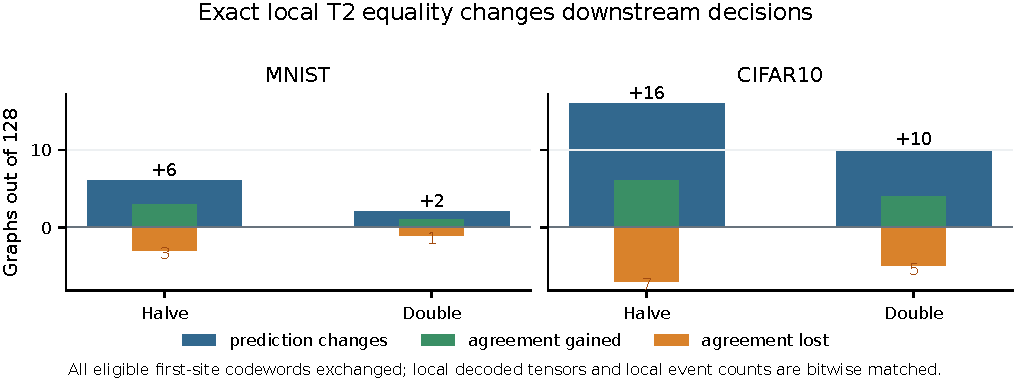
\includegraphics[width=\linewidth]{figures/temporal_decision_effects.pdf}
\caption{Exact local $T=2$ equality does not preserve paired downstream decisions. Bars count changed predictions and gained or lost teacher agreement after all eligible exchanges. Both directions preserve the local decoded tensor and event count but differ in absolute amplitude; training-only, 128 graphs per task.}
\label{fig:temporal-decisions}
\end{figure}

The same exchanges change whole-network activity: halving all eligible events raises total $T=2$ events by 3.41\% on MNIST and 4.99\% on CIFAR10, while the amplitude-increasing direction lowers CIFAR10 events by 1.33\%. Thus neither a matched local endpoint nor a fixed local event count fixes global cost. The per-graph event totals are retained in the anonymous review package.

Because the exchanged codewords have different first-prefix profiles and amplitudes, this experiment does not isolate event timing from amplitude. Its controlled statement is narrower: terminal equality plus a fixed local event count does not determine the downstream trajectory or decisions. The first-site replacement changes the signal delivered to later layers; their nonlinear event states integrate it before local equality is restored. The scalar counterexample isolates this state dependence, and the graph experiment shows that the matched terminal tensor does not fix the downstream trajectory. Likewise, lowering the first site's unweighted amplitude need not lower whole-network activity.

\subsection{Residual centering: a useful representation change with a limited guarantee}
A complementary GatedGCN diagnostic asks which part of a residual state needs event encoding. Write $h_\ell=h_0+q_\ell$ and $e_\ell=e_0+r_\ell$, where $q_\ell,r_\ell$ accumulate nonnegative residual branch increments. For a projection,
\begin{equation}
 Wh_\ell+b=(Wh_0+b)+Wq_\ell.\label{eq:center}
\end{equation}
The static carrier can be cached, and one encoded residual stream can serve the node consumers within a layer. Both compared implementations keep the first layer exact and preserve the same raw residual skip. Centering changes subsequent coded inputs from raw states to residual increments. Equation~\eqref{eq:center} is an affine identity; caching and shared streams are implementation opportunities, not new algebra.

\begin{figure}[t]
\centering
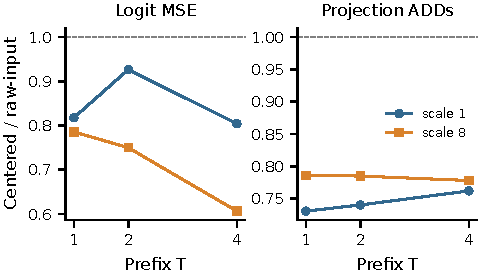
\includegraphics[width=\linewidth]{figures/centered_tradeoff.pdf}
\caption{Centering lowers the measured logit-error and projection-work ratios after an identical exact first layer. Ratios below one favor centered coding under shared channel thresholds. Full 45,000-graph CIFAR10 training split, one GatedGCN teacher; ADDs count prospective coded projections and exclude static carriers and the rest of inference.}
\label{fig:centered}
\end{figure}

Under identical shared thresholds, centering lowers logit MSE and prospective coded-projection additions at every tested prefix ($T=1,2,4$) for both threshold scales (1 and 8). At scale 1 and $T=1$, teacher agreement rises by 2.04 points, while projected additions fall from $9.099\times10^{11}$ to $6.650\times10^{11}$ across the full training split. Agreement improves in five of six comparisons, with a 0.0044-point decrease at scale 1, $T=4$. This is constructive evidence that choosing the encoded origin matters even with matched thresholds. It measures teacher fidelity and one arithmetic component for one training-split teacher, rather than test accuracy or total runtime. It also exemplifies the central distinction: a favorable representation and local work proxy still require separate decision and complete-cost validation.

A separate three-teacher campaign evaluates centered conversion on all 5,000 exposed CIFAR10 validation graphs. At $T=4/8$, centered mean accuracy is 70.53\%/70.56\%, within 0.07/0.05 points of the strongest recorded controls. However, its matched dense implementation takes 6.245/12.049 ms per graph against 6.213/3.132 for the strongest controls at those horizons. That campaign also retains nine unresolved cost-accounting items. It therefore extends the evidence for centered fidelity beyond training, while leaving a complete efficiency advantage unestablished. These controls use their own calibration and head conventions; they are kept separate from the shared-threshold training comparison in Fig.~\ref{fig:centered} and from the historical test adapters in Table~\ref{tab:main}.

\subsection{Activity, simulation time, and applicability}
Low event counts do not imply low simulation time in the primary converter. It runs dense graph projections on every tick, so zero events do not skip kernels. On an RTX 3060, synchronized cached-batch timings average 0.152/0.157 ms per graph for the MNIST/CIFAR10 ANN, versus 0.366/0.493 at $T=1$ and 1.238/1.762 at $T=4$ for the diagnostic converter. These are averages of three seed-level medians with 32-graph batches and 30 interleaved repeats; they include decoded-site accumulation, exclude transfer and loading, and are not optimized deployment bounds. No chip energy is measured.

The distinction also matters for event allocation. Actual-message allocation costs 0.834/0.991 ms per graph versus local allocation's 0.668/0.806 in its own matched timing experiment. Exact local codeword exchanges can change downstream events even when first-site counts are fixed. These measurements distinguish low $T$, local sparsity, and the projected additions in Fig.~\ref{fig:centered} from complete inference cost. A useful conversion must specify its event type, continuous work, prefix requirements, and backend.

\section{Discussion and Conclusion}
The experiments expose two scoped information losses in reconstruction-based evaluation. The measured message norm omits the signed direction of an event error relative to competing classes, while a matched local terminal tensor and event count admit different prefixes and amplitudes. Position recovery locates influential sites; hard-event changes show that improving a local metric can worsen the decision; exact codeword exchanges show that local terminal equality does not determine the downstream trajectory.

A useful design criterion follows from these distinctions. Specify the downstream quantity preserved by an approximation, then evaluate a realizable finite-event change under fixed task computation. Report teacher agreement and accuracy separately, check every required prefix, and account for whole-network activity. Residual centering and task-aware calibration illustrate why a representation identity or a decision-driven objective still requires separate decision and complete-cost validation.

The core tests concern fixed residual GCNs on superpixel graphs and use one teacher with previously used validation or training graphs. Effects on other teachers, tasks, converters, and topologies remain open, as do a matched One-Spike comparison and a feature-dependent gate perturbation study. Within these conditions, the evaluation checklist makes decision, prefix, and activity visible where message fidelity and local terminal equality do not.

\clearpage
\section*{LLM Usage Statement}
OpenAI Codex was used for research-asset inspection, analysis and experimental code, evidence checks, mathematical discussion, manuscript organization and drafting, figure-generation code, and compilation checks. Independent fresh-context reviews of the revised manuscript were conducted with Kimi K3.1 Pro and DeepSeek V4.1 Flash. Earlier project stages used WorkBuddy for research planning and execution assistance, and Claude and Grok for written reviews and suggestions. Historical records do not identify every underlying model version used in those earlier stages. The scientific results reported here originate from recorded numerical experiments and executable analyses; language-model suggestions are not treated as experimental evidence. The figures in this manuscript are programmatically rendered from recorded data or explicitly labeled mathematical examples, without generated experimental imagery. Human authors remain responsible for verifying all claims, citations, code, and disclosures and for approving any submission.

{\small
\bibliographystyle{ieeenat_fullname}
\bibliography{references}}
\end{document}
